\documentclass[11pt,a4paper]{article}

% =====================================================
% PACOTES
% =====================================================
\usepackage[utf8]{inputenc}
\usepackage[T1]{fontenc}
\usepackage[brazil]{babel}
\shorthandoff{"}
\usepackage[default]{sourcesanspro}          % texto: sem serifa, leitura confortável
\usepackage[scale=0.86]{sourcecodepro}       % código: monoespaçada moderna
\usepackage{fontawesome5}                    % ícones
\usepackage{geometry}
\usepackage{graphicx}
\usepackage{fancyhdr}
\usepackage{titlesec}
\usepackage[table]{xcolor}
\usepackage{hyperref}
\usepackage{enumitem}
\usepackage[most]{tcolorbox}
\usepackage{float}
\usepackage{tikz}
\usetikzlibrary{arrows.meta, positioning, shapes.geometric, calc, babel}
\usepackage{tabularx}
\usepackage{booktabs}
\usepackage{listings}
\usepackage{lastpage}
\usepackage{qrcode}
\usepackage{multicol}

\geometry{top=2.6cm, bottom=2.6cm, left=2cm, right=2cm, headsep=0.8cm}
\linespread{1.18}
\setlength{\parskip}{0.55em}
\setlength{\parindent}{0pt}

% =====================================================
% PALETA (cores institucionais IFSC, em tons suaves)
% =====================================================
\definecolor{azul}{RGB}{30,60,90}
\definecolor{azulMedio}{RGB}{37,99,235}
\definecolor{verde}{RGB}{22,101,52}
\definecolor{verdeVivo}{RGB}{22,163,74}
\definecolor{ambar}{RGB}{217,119,6}
\definecolor{vermelho}{RGB}{220,38,38}
\definecolor{roxo}{RGB}{124,58,237}
\definecolor{tinta}{RGB}{30,41,59}
\definecolor{suave}{RGB}{100,116,139}
\definecolor{borda}{RGB}{226,232,240}
\definecolor{fundo}{RGB}{248,250,252}
\definecolor{barraTitulo}{RGB}{241,245,249}
\definecolor{terminal}{RGB}{15,23,42}

\color{tinta}

% =====================================================
% LISTINGS
% =====================================================
\lstdefinestyle{base}{
    basicstyle=\ttfamily\small\color{tinta},
    keywordstyle=\color{azulMedio}\bfseries,
    commentstyle=\color{suave}\itshape,
    stringstyle=\color{verde},
    breaklines=true, columns=fullflexible, keepspaces=true,
    showstringspaces=false, upquote=true, tabsize=4,
    frame=none, numbers=none, aboveskip=0pt, belowskip=0pt,
    extendedchars=true,
    literate=
      {á}{{\'a}}1 {é}{{\'e}}1 {í}{{\'i}}1 {ó}{{\'o}}1 {ú}{{\'u}}1
      {Á}{{\'A}}1 {É}{{\'E}}1 {Í}{{\'I}}1 {Ó}{{\'O}}1 {Ú}{{\'U}}1
      {ã}{{\~a}}1 {õ}{{\~o}}1 {Ã}{{\~A}}1 {Õ}{{\~O}}1
      {â}{{\^a}}1 {ê}{{\^e}}1 {ô}{{\^o}}1 {Â}{{\^A}}1 {Ê}{{\^E}}1 {Ô}{{\^O}}1
      {à}{{\`a}}1 {ç}{{\c c}}1 {Ç}{{\c C}}1
      {–}{{--}}1 {±}{{$\pm$}}1 {≈}{{$\approx$}}1 {÷}{{$\div$}}1
}
\lstdefinestyle{py}{style=base, language=Python,
    morekeywords={True,False,None}}
\lstdefinestyle{tex}{style=base, language=TeX}
\lstdefinestyle{txt}{style=base}
\lstdefinestyle{saida}{style=base, language={}, basicstyle=\ttfamily\small\color{white!88!black}}
\lstset{style=base}

% =====================================================
% COMPONENTES VISUAIS
% =====================================================
% --- Janela de código (estilo editor) ---------------
\newcommand{\pontosJanela}{%
  {\color{vermelho!70}\tiny\faCircle}\,{\color{ambar!80}\tiny\faCircle}\,{\color{verdeVivo!70}\tiny\faCircle}\hspace{0.8em}}
\newtcblisting{codigo}[2][py]{
    enhanced, listing only, breakable,
    colback=fundo, colframe=borda, boxrule=0.6pt, arc=6pt,
    left=10pt, right=10pt, top=6pt, bottom=6pt,
    title={\pontosJanela #2}, coltitle=suave, colbacktitle=barraTitulo,
    fonttitle=\ttfamily\footnotesize, toptitle=2pt, bottomtitle=2pt,
    titlerule=0.6pt, titlerule style=borda,
    listing options={style=#1}
}
% --- Saída (terminal escuro) -------------------------
\newtcblisting{saida}[1][Saída]{
    enhanced, listing only, breakable,
    colback=terminal, colframe=terminal, boxrule=0pt, arc=6pt,
    left=10pt, right=10pt, top=4pt, bottom=6pt,
    title={\faTerminal\hspace{0.5em}#1}, coltitle=white!65!black,
    colbacktitle=terminal, fonttitle=\sffamily\footnotesize\bfseries,
    toptitle=3pt, bottomtitle=0pt, titlerule=0pt,
    listing options={style=saida}
}
% --- Exemplo certo/errado -----------------------------
\newtcblisting{exemplo}[2]{
    enhanced, listing only,
    colback=#1!4, colframe=#1!45, boxrule=0.6pt, arc=6pt,
    left=8pt, right=8pt, top=5pt, bottom=5pt,
    title={#2}, colbacktitle=#1!12, coltitle=#1!75!black,
    fonttitle=\sffamily\small\bfseries, toptitle=2pt, bottomtitle=2pt,
    listing options={style=py, basicstyle=\ttfamily\footnotesize\color{tinta}}
}
% --- Caixas de destaque com barra lateral -----------
\newtcolorbox{destaque}[3]{
    enhanced, breakable,
    colback=#1!6, frame hidden, arc=6pt,
    borderline west={3.5pt}{0pt}{#1},
    left=14pt, right=12pt, top=9pt, bottom=9pt,
    before upper={{\color{#1}\large #2}\hspace{0.55em}{\color{#1!75!black}\bfseries #3}\par\vspace{0.25em}}
}
\newenvironment{dica}[1]{\begin{destaque}{ambar}{\faLightbulb[regular]}{#1}}{\end{destaque}}
\newenvironment{atencao}[1]{\begin{destaque}{vermelho}{\faExclamationTriangle}{#1}}{\end{destaque}}
\newenvironment{conceito}[1]{\begin{destaque}{azulMedio}{\faBookOpen}{#1}}{\end{destaque}}
\newenvironment{sucesso}[1]{\begin{destaque}{verdeVivo}{\faCheckCircle[regular]}{#1}}{\end{destaque}}
\newenvironment{avancado}[1]{\begin{destaque}{roxo}{\faCode}{#1}}{\end{destaque}}

% --- Caixa com título "aba" (objetivos, atividade) ---
\newtcolorbox{painel}[3][]{
    enhanced, breakable,
    colback=white, colframe=borda, boxrule=0.6pt, arc=8pt,
    left=14pt, right=14pt, top=14pt, bottom=10pt,
    title={#2\hspace{0.5em}#3}, coltitle=white, colbacktitle=azul,
    fonttitle=\bfseries, attach boxed title to top left={xshift=12pt, yshift=-8pt},
    boxed title style={arc=4pt, boxrule=0pt}, #1
}
% --- Cartões pequenos ---------------------------------
\tcbset{cartao/.style={enhanced, colback=fundo, colframe=borda, boxrule=0.6pt, arc=8pt,
    left=10pt, right=10pt, top=8pt, bottom=8pt, fontupper=\small\raggedright}}

% --- Elementos em linha --------------------------------
\newcommand{\tecla}[1]{\tcbox[on line, enhanced, colback=white, colframe=suave!50, boxrule=0.5pt,
    arc=2.5pt, left=3pt, right=3pt, top=0.5pt, bottom=0.5pt, boxsep=0.5pt,
    borderline south={1.2pt}{0pt}{suave!40}]{\ttfamily\footnotesize #1}}
\newcommand{\botao}[1]{\tcbox[on line, enhanced, colback=azulMedio!8, colframe=azulMedio!35, boxrule=0.5pt,
    arc=3pt, left=3pt, right=3pt, top=0.5pt, bottom=0.5pt, boxsep=0.5pt]{\sffamily\footnotesize\color{azul}#1}}
\newcommand{\seta}{\,{\color{suave}\scriptsize\faChevronRight}\,}
\newcommand{\chip}[2]{\tcbox[on line, enhanced, colback=white, opacityback=0.14, colframe=white,
    opacityframe=0.45, boxrule=0.5pt, arc=8pt, left=5pt, right=5pt, top=1.5pt, bottom=1.5pt,
    boxsep=0pt, coltext=white]{\footnotesize #1\hspace{0.4em}#2}}
\newcommand{\circulo}[2][azul]{\tikz[baseline=(c.base)]\node[circle, fill=#1, text=white,
    inner sep=0pt, minimum size=1.35em, font=\footnotesize\bfseries](c){#2};}
\newcommand{\marca}[1]{\tikz[baseline=(c.base)]\node[circle, fill=vermelho, text=white,
    inner sep=0pt, minimum size=1.2em, font=\scriptsize\bfseries](c){#1};}
\newcommand{\caixaMarcar}{{\color{suave}\faSquare[regular]}}

% =====================================================
% HIPERLINKS
% =====================================================
\hypersetup{colorlinks=true, linkcolor=azulMedio, urlcolor=verde, citecolor=azul}
\newcommand{\urlKit}{https://chameoandre.github.io/CST-Sistemas-para-internet-iniciacao-cientifica-extensionista/2026-2/roteiro-2-python-graficos}
\newcommand{\urlColab}{https://colab.research.google.com/github/chameoandre/CST-Sistemas-para-internet-iniciacao-cientifica-extensionista/blob/main/2026-2/roteiro-2-python-graficos/analise_experimento.ipynb}

% =====================================================
% CABEÇALHO E RODAPÉ
% =====================================================
\pagestyle{fancy}
\fancyhf{}
\fancyhead[L]{%
    \IfFileExists{figures/garopaba_horizontal_marca2015_PNG.png}{%
        \raisebox{-0.25\height}{
\includegraphics[height=0.95cm]{figures/garopaba_horizontal_marca2015_PNG.png}}%
    }{\textbf{\color{verde} IFSC — Câmpus Garopaba}}}
\fancyhead[R]{\footnotesize\color{suave}\textbf{\color{azul}Roteiro Prático 02}\hspace{0.5em}\textbullet\hspace{0.5em}Starter Kit Python \& Gráficos}
\fancyfoot[L]{\footnotesize\color{suave}Iniciação Científica e Extensionista\hspace{0.4em}\textbullet\hspace{0.4em}CST Sistemas para a Internet}
\fancyfoot[R]{\tcbox[on line, colback=azul!8, colframe=azul!8, arc=6pt, boxrule=0pt, left=5pt, right=5pt, top=1pt, bottom=1pt, boxsep=0pt]{\footnotesize\color{azul}\bfseries\thepage\,/\,\pageref*{LastPage}}}
\renewcommand{\headrule}{{\color{borda}\hrule height 0.6pt}}
\renewcommand{\footrulewidth}{0pt}
\setlength{\headheight}{36pt}

% =====================================================
% TÍTULOS DE SEÇÃO
% =====================================================
\titleformat{\section}
  {\normalfont\Large\bfseries\color{azul}}
  {\tikz[baseline=(n.base)]\node[fill=azul, rounded corners=5pt, text=white, inner sep=5pt,
      minimum width=1.9em, font=\large\bfseries](n){\thesection};}
  {0.7em}{}
\titlespacing*{\section}{0pt}{1.6em}{0.7em}

\titleformat{\subsection}
  {\normalfont\large\bfseries\color{azul!85!black}}
  {{\color{verdeVivo}\thesubsection}}
  {0.6em}{}
\titlespacing*{\subsection}{0pt}{1.2em}{0.4em}

\setlist[itemize]{leftmargin=1.4em, itemsep=0.25em, topsep=0.3em, label={\color{verdeVivo}\small\faAngleRight}}
\setlist[enumerate]{leftmargin=2.2em, itemsep=0.45em, topsep=0.3em}

% Tabelas: sem linhas verticais, cabeçalho colorido, zebra suave
\newcommand{\cabecalho}{\rowcolor{azul}}
\newcommand{\cab}[1]{\leavevmode\color{white}\bfseries #1}
\arrayrulecolor{borda}
\newcolumntype{Y}{>{\raggedright\arraybackslash}X}
\newcolumntype{P}[1]{>{\raggedright\arraybackslash}p{#1}}

\begin{document}

% =====================================================
% CAPA / BANNER
% =====================================================
\begin{tcolorbox}[enhanced, frame hidden, arc=12pt,
    interior style={left color=azul, right color=verde},
    left=20pt, right=20pt, top=18pt, bottom=16pt, colupper=white,
    overlay={\node[anchor=east, opacity=0.13, font=\fontsize{90}{90}\selectfont, text=white] at ([xshift=-14pt]frame.east) {\faChartBar};}]
{\footnotesize\bfseries\color{white!80!azul}ROTEIRO PRÁTICO 02\hspace{0.6em}\textbullet\hspace{0.6em}INICIAÇÃO CIENTÍFICA E EXTENSIONISTA}\par\vspace{2pt}
{\fontsize{25}{30}\selectfont\bfseries Starter Kit Python \& Gráficos}\par\vspace{2pt}
{\large Dos dados coletados às figuras e tabelas do artigo no Overleaf}\par\vspace{10pt}
\chip{\faSeedling}{Nível iniciante}\hspace{4pt}
\chip{\faTools}{Google Colab · Python · Overleaf}\hspace{4pt}
\chip{\faLink}{Pré-requisito: Roteiro 01}
\end{tcolorbox}

\vspace{0.4em}

\begin{tcbraster}[raster columns=3, raster equal height, raster column skip=8pt]
\begin{tcolorbox}[cartao]
{\color{azulMedio}\faUniversity}\hspace{0.4em}\textbf{Unidade Curricular}\par\vspace{2pt}
Iniciação Científica e Extensionista\\ {\color{suave}60h / 30h CHCE}
\end{tcolorbox}
\begin{tcolorbox}[cartao]
{\color{azulMedio}\faChalkboardTeacher}\hspace{0.4em}\textbf{Docentes}\par\vspace{2pt}
Prof. Dr. André Moraes\\ Prof. Dr. Adalberto Tabalipa
\end{tcolorbox}
\begin{tcolorbox}[cartao]
{\color{azulMedio}\faFlag}\hspace{0.4em}\textbf{Produto final da UC}\par\vspace{2pt}
Artigo científico submetido ao \textit{Computer on the Beach} (COTB 2027)
\end{tcolorbox}
\end{tcbraster}

\vspace{0.6em}

\begin{painel}{\faBullseye}{Ao final desta prática você será capaz de\ldots}
\begin{itemize}
    \item \textbf{Usar o Google Colab} para abrir, executar e salvar um notebook Python --- mesmo que nunca tenha programado;
    \item \textbf{Organizar os dados} da pesquisa/ação extensionista em um arquivo \texttt{.csv} no formato ``uma linha por medição'';
    \item \textbf{Calcular estatísticas descritivas} por grupo: número de observações ($n$), média, desvio padrão, mínimo e máximo;
    \item \textbf{Escolher o gráfico adequado} à pergunta de pesquisa e exportá-lo em \textbf{PDF vetorial} no tamanho de uma coluna ACM;
    \item \textbf{Gerar uma tabela \LaTeX{}} no padrão \texttt{booktabs} e integrá-la ao artigo no Overleaf;
    \item \textbf{Descrever os resultados} com citação cruzada, interpretando --- e não apenas repetindo --- os números.
\end{itemize}
\end{painel}

\vspace{0.4em}

{\large\bfseries\color{azul}\faMap[regular]\hspace{0.5em}Mapa da aula}\par\vspace{0.2em}
\begin{tcbraster}[raster columns=2, raster equal height, raster column skip=8pt, raster row skip=6pt]
\begin{tcolorbox}[cartao, colback=azulMedio!5, colframe=azulMedio!25]
\circulo[azulMedio]{1}\hspace{0.4em}\textbf{Conhecer o Colab}\par\vspace{2pt}
{\color{suave}\footnotesize Interface, células e aquecimento (Seções~\ref{sec:colab} e~\ref{sec:python})}
\end{tcolorbox}
\begin{tcolorbox}[cartao, colback=verdeVivo!5, colframe=verdeVivo!25]
\circulo[verdeVivo]{2}\hspace{0.4em}\textbf{Rodar o kit}\par\vspace{2pt}
{\color{suave}\footnotesize Notebook com os dados de exemplo (Seção~\ref{sec:kit})}
\end{tcolorbox}
\begin{tcolorbox}[cartao, colback=ambar!6, colframe=ambar!30]
\circulo[ambar]{3}\hspace{0.4em}\textbf{Usar seus dados}\par\vspace{2pt}
{\color{suave}\footnotesize CSV da dupla e escolha do gráfico (Seções~\ref{sec:dados} a~\ref{sec:grafico})}
\end{tcolorbox}
\begin{tcolorbox}[cartao, colback=roxo!5, colframe=roxo!25]
\circulo[roxo]{4}\hspace{0.4em}\textbf{Escrever}\par\vspace{2pt}
{\color{suave}\footnotesize Figura, tabela e texto no Overleaf (Seções~\ref{sec:overleaf} a~\ref{sec:atividade})}
\end{tcolorbox}
\end{tcbraster}

% =====================================================
% 1. ONDE ESTE ROTEIRO SE ENCAIXA
% =====================================================
\section{Onde este roteiro se encaixa}\label{sec:pipeline}

No Roteiro 01 preparamos o \textbf{esqueleto do artigo} no Overleaf. Agora vamos produzir o seu conteúdo mais importante: a \textbf{evidência}. Os dados coletados (questionários, medições, auditorias de sites, registros da ação extensionista) passam por um pequeno programa em Python que gera, automaticamente, as figuras e a tabela da seção de \textit{Resultados}.

\begin{center}
\begin{tikzpicture}[node distance=0.42cm,
    etapa/.style={rectangle, draw=borda, fill=fundo, line width=0.6pt, text width=2.55cm, align=center,
        rounded corners=7pt, minimum height=2.15cm, font=\footnotesize},
    linha/.style={draw=suave!70, -{Latex[length=2.2mm]}, line width=0.9pt}]
    \node[etapa] (coleta) {{\color{azulMedio}\Large\faClipboardList}\\[3pt]\textbf{Coleta}\\{\color{suave}formulários, medições}};
    \node[etapa, right=of coleta] (csv) {{\color{azulMedio}\Large\faTable}\\[3pt]\textbf{Planilha}\\{\color{suave}salva como \texttt{.csv}}};
    \node[etapa, right=of csv, draw=verdeVivo, fill=verdeVivo!7, line width=1.1pt] (py) {{\color{verdeVivo}\Large\faPython}\\[3pt]\textbf{Python no Colab}\\{\color{suave}este roteiro}};
    \node[etapa, right=of py] (saida) {{\color{azulMedio}\Large\faChartBar}\\[3pt]\textbf{Saídas}\\{\color{suave}gráficos \texttt{.pdf} e tabela \texttt{.tex}}};
    \node[etapa, right=of saida] (ov) {{\color{azulMedio}\Large\faLeaf}\\[3pt]\textbf{Overleaf}\\{\color{suave}seção de Resultados}};
    \draw[linha] (coleta) -- (csv);
    \draw[linha] (csv) -- (py);
    \draw[linha] (py) -- (saida);
    \draw[linha] (saida) -- (ov);
\end{tikzpicture}
\end{center}

\begin{dica}{Por que usar um programa em vez de fazer o gráfico no Excel/Planilhas?}
\begin{itemize}
    \item \textbf{Reprodutibilidade:} se um dado mudar (ou um revisor pedir uma correção), basta executar de novo --- todas as figuras e a tabela são refeitas idênticas, em segundos;
    \item \textbf{Qualidade gráfica:} o PDF vetorial não perde nitidez com zoom nem na impressão dos anais;
    \item \textbf{Padronização:} todas as figuras do artigo saem com a mesma fonte, tamanho e cores.
\end{itemize}
\end{dica}

% =====================================================
% 2. PRIMEIROS PASSOS NO GOOGLE COLAB
% =====================================================
\section{Primeiros passos no Google Colab}\label{sec:colab}

\subsection{O que é o Google Colab?}

O \textbf{Google Colab} (\textit{Colaboratory}) é um serviço gratuito do Google para escrever e executar programas em \textbf{Python} diretamente no navegador. Pense nele como um \textbf{``Google Docs para programar''}: o arquivo fica salvo no seu Google Drive, pode ser compartilhado por link e o código é executado nos computadores do Google --- e não no seu.

\begin{tcbraster}[raster columns=3, raster equal height, raster column skip=8pt]
\begin{tcolorbox}[cartao]
{\color{verdeVivo}\Large\faLaptop}\par\vspace{2pt}
\textbf{Nada para instalar}\par
{\color{suave}Funciona em qualquer computador com navegador (Chrome, Firefox, Edge\ldots).}
\end{tcolorbox}
\begin{tcolorbox}[cartao]
{\color{verdeVivo}\Large\faGoogleDrive}\par\vspace{2pt}
\textbf{Basta uma conta Google}\par
{\color{suave}O notebook é salvo no seu Drive, como um documento comum.}
\end{tcolorbox}
\begin{tcolorbox}[cartao]
{\color{verdeVivo}\Large\faBoxOpen}\par\vspace{2pt}
\textbf{Bibliotecas prontas}\par
{\color{suave}\texttt{pandas} e \texttt{matplotlib}, usadas neste roteiro, já vêm instaladas.}
\end{tcolorbox}
\end{tcbraster}

\subsection{Vocabulário mínimo}

\begin{center}
\small
\renewcommand{\arraystretch}{1.45}
\rowcolors{2}{fundo}{white}
\begin{tabularx}{\linewidth}{>{\raggedright\arraybackslash\bfseries\leavevmode\color{azul}}p{4.1cm}Y}
\cabecalho \cab{Termo} & \cab{O que significa} \\
Notebook (\texttt{.ipynb}) & O arquivo do Colab. Mistura textos explicativos, código e os resultados do código, como um caderno de laboratório. \\
Célula & Cada bloco do notebook. Há dois tipos: \textbf{células de texto} (explicações) e \textbf{células de código} (instruções em Python). \\
Executar uma célula & Pedir ao computador que realize as instruções daquela célula. O resultado aparece logo abaixo dela (a \textbf{saída}). \\
Ambiente de execução (sessão) & O computador do Google ``emprestado'' para você enquanto o notebook está aberto. É temporário! \\
Biblioteca & Um conjunto de ferramentas prontas. Usamos o \texttt{pandas} (tabelas) e o \texttt{matplotlib} (gráficos). \\
CSV & ``Valores separados por vírgula'': um formato simples de planilha, que qualquer programa consegue ler. \\
DataFrame & Uma tabela carregada na memória pelo \texttt{pandas}, com linhas e colunas --- como uma aba de planilha. \\
\end{tabularx}
\end{center}

\subsection{Conhecendo a tela}\label{sec:tela}

A Figura~\ref{fig:tela} mostra um esquema simplificado da tela do Colab. Os números em vermelho correspondem à legenda logo abaixo da figura.

\begin{figure}[H]
\centering
\begin{tikzpicture}[x=1cm, y=1cm, font=\sffamily\footnotesize]
    % janela
    \draw[borda, line width=0.8pt, fill=white, rounded corners=8pt] (0,0) rectangle (16.6,8.6);
    % barra do título
    \begin{scope}
        \clip[rounded corners=8pt] (0,0) rectangle (16.6,8.6);
        \fill[barraTitulo] (0,7.85) rectangle (16.6,8.6);
    \end{scope}
    \node[anchor=west, font=\sffamily\small\bfseries, text=tinta] at (0.35,8.22) {{\color{ambar}\faBook}\hspace{0.4em}Cópia de analise\_experimento.ipynb};
    \node[anchor=east] at (16.3,8.22) {\tcbox[on line, colback=azulMedio!10, colframe=azulMedio!30, boxrule=0.4pt, arc=8pt, left=5pt, right=5pt, top=0pt, bottom=0pt]{\footnotesize\color{azul}\faUserPlus\ Compartilhar}};
    % menu
    \node[anchor=west, text=tinta] at (0.35,7.5) {Arquivo\quad Editar\quad Ver\quad Inserir\quad \textbf{Ambiente de execução}\quad Ferramentas\quad Ajuda};
    \draw[borda] (0,7.18) -- (16.6,7.18);
    % barra de ferramentas
    \node[anchor=west] at (1.15,6.8) {\botao{+ Código}\ \botao{+ Texto}};
    \node[anchor=east] at (16.3,6.8) {\tcbox[on line, colback=verdeVivo!10, colframe=verdeVivo!40, boxrule=0.4pt, arc=3pt, left=4pt, right=4pt, top=0pt, bottom=0pt]{\footnotesize\color{verde}\faCheck\ RAM \rule[1pt]{0.7cm}{2pt}\ Disco \rule[1pt]{0.5cm}{2pt}}};
    \draw[borda] (0,6.45) -- (16.6,6.45);
    % barra lateral
    \draw[borda] (0.85,0) -- (0.85,6.45);
    \node[text=suave] at (0.42,5.95) {\faListUl};
    \node[text=suave] at (0.42,5.25) {\faSearch};
    \node[text=suave] at (0.42,4.55) {\faKey};
    \node[fill=azulMedio!12, rounded corners=3pt, text=azulMedio, minimum size=0.55cm] at (0.42,3.85) {\faFolder};
    % célula de texto
    \node[anchor=west, font=\sffamily\large\bfseries, text=tinta] at (1.4,5.85) {Roteiro Prático 02 --- Starter Kit};
    \node[anchor=west, text=suave] at (1.4,5.35) {Execute as células em ordem com Shift + Enter.};
    % célula de código 1
    \draw[borda, fill=fundo, rounded corners=4pt] (1.3,3.55) rectangle (16.1,4.8);
    \node[circle, fill=tinta, text=white, minimum size=0.55cm, inner sep=0pt] at (1.75,4.45) {\scriptsize\faPlay};
    \node[anchor=west, font=\ttfamily\footnotesize, align=left, text=tinta] at (2.25,4.17)
        {{\color{azulMedio}\bfseries import} pandas {\color{azulMedio}\bfseries as} pd\\print({\color{verde}\textquotedbl Olá, IFSC Garopaba!\textquotedbl})};
    % saída
    \node[anchor=west, font=\ttfamily\footnotesize, text=tinta] at (2.25,3.15) {Olá, IFSC Garopaba!};
    % célula de código 2 (não executada)
    \draw[borda, fill=fundo, rounded corners=4pt] (1.3,1.05) rectangle (16.1,2.55);
    \node[text=suave, font=\ttfamily\footnotesize] at (1.75,2.2) {[ ]};
    \node[anchor=west, font=\ttfamily\footnotesize, align=left, text=tinta] at (2.25,1.8)
        {notas = [7.5, 8.0, 9.5, 6.0]\\print(sum(notas) / len(notas))};
    % marcadores numerados
    \node at (11.55,7.5) {\marca{1}};
    \node at (4.45,6.8) {\marca{2}};
    \node at (11.6,6.8) {\marca{3}};
    \node at (0.42,3.2) {\marca{4}};
    \node at (8.4,5.85) {\marca{5}};
    \node at (1.75,3.85) {\marca{6}};
    \node at (5.8,3.15) {\marca{7}};
    \node at (1.75,0.65) {\marca{8}};
\end{tikzpicture}
\caption{Esquema da tela do Google Colab (representação simplificada).}
\label{fig:tela}
\end{figure}

\begin{multicols}{2}
\small
\begin{itemize}[label={}, leftmargin=0pt, itemsep=0.35em]
    \item \marca{1}\ \textbf{Menu.} Em \textit{Arquivo} você salva uma cópia; em \textit{Ambiente de execução} você executa ou reinicia tudo.
    \item \marca{2}\ \textbf{+ Código / + Texto:} insere uma nova célula de código ou de texto.
    \item \marca{3}\ \textbf{Conexão.} Quando aparece \textit{RAM/Disco}, você está conectado a um computador do Google. Se aparecer \textit{Conectar}, clique nele.
    \item \marca{4}\ \textbf{Arquivos.} O ícone de pasta abre o painel para enviar (\textit{upload}) e baixar (\textit{download}) arquivos.
    \item \marca{5}\ \textbf{Célula de texto:} explicações. Dê dois cliques para editar.
    \item \marca{6}\ \textbf{Botão executar} (\faPlay): roda a célula de código. Atalho: \tecla{Shift}+\tecla{Enter}.
    \item \marca{7}\ \textbf{Saída:} o resultado aparece logo abaixo da célula executada.
    \item \marca{8}\ \textbf{\texttt{[ ]} vazio:} a célula ainda \textbf{não foi executada}. Depois de executada, mostra um número (\texttt{[1]}, \texttt{[2]}\ldots) que indica a ordem de execução.
\end{itemize}
\end{multicols}

\subsection{Mão na massa: aquecimento de 10 minutos}\label{sec:aquecimento}

Antes de usar o kit, vamos criar um notebook de teste para perder o medo. Nada do que você fizer aqui pode ``estragar'' o computador.

\begin{enumerate}[label={\protect\circulo{\arabic*}}]
    \item Acesse \href{https://colab.research.google.com}{\texttt{colab.research.google.com}} e faça login com sua conta Google.
    \item Na janela que se abre, clique em \botao{+ Novo notebook} (ou \botao{Arquivo}\seta\botao{Novo notebook no Drive}).
    \item Clique no título \texttt{Untitled0.ipynb}, no alto, e renomeie para \texttt{aquecimento.ipynb}.
    \item Digite na primeira célula o código abaixo e pressione \tecla{Shift}+\tecla{Enter}. A primeira execução pode demorar alguns segundos, porque o Colab está se conectando.
\end{enumerate}

\begin{codigo}{Célula 1}
print("Olá, IFSC Garopaba!")
\end{codigo}
\begin{saida}
Olá, IFSC Garopaba!
\end{saida}

\begin{enumerate}[label={\protect\circulo{\arabic*}}, start=5]
    \item O \tecla{Shift}+\tecla{Enter} já levou você para a célula seguinte. Faça uma conta --- o Colab mostra automaticamente o resultado da \textbf{última linha} da célula:
\end{enumerate}

\begin{codigo}{Célula 2}
2 + 3 * 4
\end{codigo}
\begin{saida}
14
\end{saida}

\begin{enumerate}[label={\protect\circulo{\arabic*}}, start=6]
    \item Agora guarde valores em \textbf{variáveis} (nomes que guardam um valor) e calcule uma média:
\end{enumerate}

\begin{codigo}{Célula 3}
notas = [7.5, 8.0, 9.5, 6.0]          # uma lista de números
media = sum(notas) / len(notas)       # soma ÷ quantidade
print("Média da turma:", media)
\end{codigo}
\begin{saida}
Média da turma: 7.75
\end{saida}

\begin{enumerate}[label={\protect\circulo{\arabic*}}, start=7]
    \item Por fim, \textbf{provoque um erro de propósito} (digitando \texttt{medis} em vez de \texttt{media}) para aprender a ler a mensagem:
\end{enumerate}

\begin{codigo}{Célula 4}
print(medis)
\end{codigo}
\begin{saida}[Saída (erro)]
NameError                                 Traceback (most recent call last)
----> 1 print(medis)
NameError: name 'medis' is not defined. Did you mean: 'media'?
\end{saida}

\begin{conceito}{Como ler uma mensagem de erro}
Leia sempre a \textbf{última linha}: ela diz o \textbf{tipo} do erro (\texttt{NameError}) e o \textbf{motivo} (o nome \texttt{medis} não existe). Muitas vezes o próprio Python sugere a correção (\textit{Did you mean: 'media'?}). Errar faz parte: corrija e execute a célula de novo. O Colab também pode exibir um botão para \textbf{explicar o erro com IA} --- use como apoio, mas confira se você entendeu o motivo.
\end{conceito}

\subsection{Regras de ouro do Colab}\label{sec:regras}

\begin{tcbraster}[raster columns=2, raster equal height, raster column skip=8pt, raster row skip=8pt]
\begin{tcolorbox}[cartao]
{\color{azulMedio}\faSortNumericDown}\hspace{0.4em}\textbf{A ordem importa}\par\vspace{2pt}
Execute as células \textbf{de cima para baixo}. Se uma célula usa algo criado em outra, a anterior precisa ter sido executada antes. Na dúvida: \botao{Ambiente de execução}\seta\botao{Executar tudo}.
\end{tcolorbox}
\begin{tcolorbox}[cartao]
{\color{vermelho}\faHourglassHalf}\hspace{0.4em}\textbf{Arquivos enviados são temporários}\par\vspace{2pt}
Tudo o que está no painel \faFolder\ é \textbf{apagado quando a sessão termina} (ao fechar a aba ou após um tempo parado). \textbf{Baixe os gráficos assim que forem gerados!}
\end{tcolorbox}
\begin{tcolorbox}[cartao]
{\color{verdeVivo}\faSave[regular]}\hspace{0.4em}\textbf{O notebook fica salvo no Drive}\par\vspace{2pt}
O código e os textos são salvos automaticamente (pasta \textit{Colab Notebooks} do seu Drive). Ao reabrir, basta \textbf{executar tudo de novo}.
\end{tcolorbox}
\begin{tcolorbox}[cartao]
{\color{ambar}\faRedo}\hspace{0.4em}\textbf{Travou? Reinicie}\par\vspace{2pt}
Se algo estranho acontecer: \botao{Ambiente de execução}\seta\botao{Reiniciar sessão} e depois \botao{Executar tudo}. Uma célula com o ícone girando ainda está executando --- aguarde.
\end{tcolorbox}
\end{tcbraster}

% =====================================================
% 3. PYTHON MÍNIMO
% =====================================================
\section{Python mínimo: o suficiente para editar o kit}\label{sec:python}

Você \textbf{não precisa} aprender a programar para usar o kit. Só vai alterar algumas linhas de \textbf{configuração} no início do código. Para isso, basta conhecer cinco regras:

\begin{enumerate}[label={\protect\circulo[verdeVivo]{\arabic*}}]
    \item \textbf{Variável = nome que guarda um valor.} Em \texttt{COLUNA\_GRUPO = "portal"}, o nome fica à esquerda do \texttt{=} e o valor, à direita. Altere \textbf{apenas o valor}.
    \item \textbf{Texto sempre entre aspas:} \texttt{"portal"}. Números \textbf{sem aspas} e com \textbf{ponto} decimal: \texttt{3.33} (e não \texttt{3,33}).
    \item \textbf{O que vem depois de \texttt{\#} é comentário:} o Python ignora. Serve para explicar o código a quem lê.
    \item \textbf{Maiúsculas e minúsculas importam:} \texttt{"Portal"} é diferente de \texttt{"portal"}. Os nomes de coluna devem ser idênticos aos do seu CSV.
    \item \textbf{Não apague símbolos} como aspas de fechamento, parênteses e vírgulas que separam itens. \texttt{None} (sem aspas) significa ``nenhum valor''.
\end{enumerate}

\begin{tcbraster}[raster columns=2, raster equal height, raster column skip=8pt]
\begin{exemplo}{verdeVivo}{\faCheckCircle\ Certo}
COLUNA_GRUPO = "portal"
LARGURA_COLUNA_POL = 3.33
COLUNA_METRICA = "acessibilidade"
ROTULO_EIXO_Y = "Pontuação (0–100)"
\end{exemplo}
\begin{exemplo}{vermelho}{\faTimesCircle\ Errado}
COLUNA_GRUPO = portal       # sem aspas
LARGURA_COLUNA_POL = 3,33   # vírgula decimal
COLUNA_METRICA = "Acessibilidade"  # maiúscula
ROTULO_EIXO_Y = "Pontuação (0–100)  # sem fechar
\end{exemplo}
\end{tcbraster}

% =====================================================
% 4. ABRINDO O STARTER KIT
% =====================================================
\section{Abrindo e executando o Starter Kit}\label{sec:kit}

\begin{tcolorbox}[enhanced, colback=verdeVivo!5, colframe=verdeVivo!30, boxrule=0.6pt, arc=8pt, left=12pt, right=12pt, top=10pt, bottom=10pt, sidebyside, lefthand ratio=0.79, sidebyside gap=14pt, segmentation hidden]
{\color{verde}\bfseries\faBoxOpen\hspace{0.5em}Arquivos do Starter Kit}\par\vspace{2pt}
\small
\begin{tabularx}{\linewidth}{>{\ttfamily}lY}
analise\_experimento.ipynb & Notebook para o Colab, com o código dividido em células comentadas \\
analise\_experimento.py & O mesmo código em um único arquivo (para o VS Code) \\
dados\_experimento.csv & Dados de exemplo: acessibilidade de 5 portais, 5 medições cada \\
\end{tabularx}\par\vspace{3pt}
{\color{suave}Pasta do kit:} \href{\urlKit/}{\texttt{2026-2/roteiro-2-python-graficos/}}
\tcblower
\centering
\qrcode[height=2.3cm]{\urlColab}\par\vspace{3pt}
{\scriptsize\color{suave}Abrir no Colab}
\end{tcolorbox}

\subsection{Executando com os dados de exemplo}

\begin{enumerate}[label={\protect\circulo{\arabic*}}]
    \item Abra o notebook pelo link direto (ou leia o QR Code acima):\\
    \href{\urlColab}{\faExternalLink*\ \texttt{Abrir analise\_experimento.ipynb no Google Colab}}
    \item O Colab exibirá o aviso \textit{``Este notebook não foi criado pelo Google''}. Como este é o notebook oficial da disciplina, clique em \botao{Executar mesmo assim}.
    \item Clique em \botao{Arquivo}\seta\botao{Salvar uma cópia no Drive}.\newline Uma nova aba se abre com o título ``Cópia de analise\_experimento'': \textbf{trabalhe sempre nesta cópia} --- é ela que guarda as suas alterações.
    \item Leia as células de texto e execute as de código, uma a uma, com \tecla{Shift}+\tecla{Enter} (ou tudo de uma vez: \botao{Ambiente de execução}\seta\botao{Executar tudo}).
    \item Observe as saídas: a tabela de estatísticas e os dois gráficos aparecem abaixo das respectivas células.
    \item Abra o painel de arquivos (\faFolder, na barra lateral esquerda). Em cada arquivo gerado, clique nos três pontinhos (\faEllipsisV)\seta\botao{Fazer download}.
\end{enumerate}

\begin{atencao}{Cuidado com notebooks desconhecidos}
O aviso do passo 2 existe por segurança: um notebook pode executar qualquer código na sua conta. Clique em \textit{Executar mesmo assim} apenas em notebooks de fontes confiáveis, como o repositório da disciplina.
\end{atencao}

\subsection{Executando com os dados da sua dupla}

\begin{enumerate}[label={\protect\circulo[ambar]{\arabic*}}]
    \item No painel \faFolder, clique no ícone de envio (\faUpload\ \textit{Fazer upload para o armazenamento da sessão}) e escolha o seu \texttt{.csv} --- ou simplesmente arraste o arquivo para o painel.
    \item Na célula \textbf{CONFIGURAÇÃO}, altere \texttt{ARQUIVO\_DADOS} para o nome exato do seu arquivo e ajuste os nomes das colunas (Seção~\ref{sec:script}).
    \item Execute tudo novamente: \botao{Ambiente de execução}\seta\botao{Executar tudo}.
    \item Baixe os novos gráficos e a tabela. Lembre-se: o \texttt{.csv} enviado some ao final da sessão --- guarde o original no seu computador ou Drive.
\end{enumerate}

\begin{avancado}{Para quem já programa: VS Code ou terminal}
Com o Python 3 instalado, execute na pasta do \texttt{.py} e do \texttt{.csv}:\par\vspace{2pt}
\texttt{python -m pip install pandas matplotlib}\\
\texttt{python analise\_experimento.py}
\end{avancado}

% =====================================================
% 5. ORGANIZANDO OS DADOS
% =====================================================
\section{Organizando os dados: ``uma linha por medição''}\label{sec:dados}

O erro mais comum na análise de dados não está no código, e sim na \textbf{planilha}. Para que o kit funcione com qualquer tema, organize os dados assim:

\begin{itemize}
    \item \textbf{cada linha} é uma observação (uma resposta de questionário, uma medição, uma rodada de teste);
    \item \textbf{cada coluna} é uma variável (o grupo comparado, o número da rodada, a métrica medida);
    \item a \textbf{primeira linha} contém os nomes das colunas --- curtos, sem acentos e sem espaços.
\end{itemize}

\begin{codigo}[txt]{dados\_experimento.csv}
portal,rodada,acessibilidade,tempo_carregamento_s
Portal A,1,86,2.20
Portal A,2,82,2.66
...
Portal E,5,93,4.28
\end{codigo}

No exemplo da disciplina, uma dupla auditou a \textbf{acessibilidade} de 5 portais públicos com o Lighthouse, repetindo a medição \textbf{5 vezes} em cada portal. A coluna \texttt{portal} é o \textbf{grupo} e a coluna \texttt{acessibilidade} é a \textbf{métrica}. O mesmo formato serve para outros temas: \texttt{turma}\,$\times$\,\texttt{nota}, \texttt{aplicativo}\,$\times$\,\texttt{tempo\_tarefa\_s}, \texttt{faixa\_etaria}\,$\times$\,\texttt{satisfacao} etc.

\begin{dica}{Exportando do Google Forms, Google Planilhas ou Excel}
\begin{itemize}
    \item \textbf{Google Forms:} na aba \textit{Respostas}, clique em \botao{Vincular ao Planilhas}. Depois, na planilha: \botao{Arquivo}\seta\botao{Fazer download}\seta\botao{Valores separados por vírgula (.csv)};
    \item \textbf{Excel em português:} o \texttt{.csv} costuma sair com \textbf{ponto e vírgula} (\texttt{;}) como separador e \textbf{vírgula} decimal (\texttt{2,20}). Nesse caso, ajuste no kit: \texttt{SEPARADOR = ";"} e \texttt{DECIMAL = ","};
    \item \textbf{Nunca} misture texto e número na mesma coluna (ex.: \texttt{"2,2 s"}). Coloque a unidade no \textbf{nome} da coluna: \texttt{tempo\_carregamento\_s}.
\end{itemize}
\end{dica}

% =====================================================
% 6. O SCRIPT EM 5 BLOCOS
% =====================================================
\section{Entendendo o código em 5 blocos}\label{sec:script}

A única parte que você \textbf{precisa} alterar é a configuração. Mesmo assim, entender o que cada bloco faz é essencial para \textbf{descrever a metodologia de análise} no artigo.

\begin{codigo}{Configuração --- a única parte que você altera}
ARQUIVO_DADOS  = "dados_experimento.csv"  # seu CSV
COLUNA_GRUPO   = "portal"                 # grupos comparados
COLUNA_METRICA = "acessibilidade"         # coluna numérica analisada
ROTULO_EIXO_Y  = "Pontuação de acessibilidade (0–100)"  # com unidade!
LIMITE_Y       = (0, 105)                 # ou None (escala automática)
\end{codigo}

\subsection*{\circulo{1}\hspace{0.4em}Carregar os dados}
O \texttt{pandas} lê o \texttt{.csv} e cria uma tabela na memória (\textit{DataFrame}). As primeiras linhas são exibidas para você conferir se a leitura está correta. Se o arquivo não for encontrado, o kit usa os dados de exemplo e avisa.

\begin{codigo}{Bloco 1}
df = pd.read_csv(origem, sep=SEPARADOR, decimal=DECIMAL)
print(df.head())     # mostra as 5 primeiras linhas
\end{codigo}

\subsection*{\circulo{2}\hspace{0.4em}Estatísticas descritivas por grupo}
Uma única instrução agrupa as medições e calcula, para cada grupo, $n$, média, desvio padrão, mínimo e máximo:

\begin{codigo}{Bloco 2}
resumo = (df.groupby(COLUNA_GRUPO)[COLUNA_METRICA]
            .agg(n="count", media="mean", desvio="std",
                 minimo="min", maximo="max")
            .reset_index())
\end{codigo}
\begin{saida}
  portal  n  media  desvio  minimo  maximo
Portal A  5   87.0    3.32      82      91
Portal B  5   62.4    2.30      60      66
Portal C  5   93.4    1.14      92      95
Portal D  5   70.4    3.91      66      75
Portal E  5   86.6    5.32      80      93
\end{saida}

\subsection*{\circulo{3}\hspace{0.2em}\circulo{4}\hspace{0.4em}Gráficos no tamanho exato de uma coluna}
A largura de \textbf{uma coluna} do template ACM \texttt{sigconf} é de aproximadamente \textbf{3,33 polegadas} (8,45\,cm). Por isso a figura já é criada nesse tamanho: se você gerar um gráfico grande e o \LaTeX{} reduzi-lo para caber na coluna, \textbf{as letras ficam minúsculas e ilegíveis}.

\begin{codigo}{Blocos 3 e 4}
fig, ax = plt.subplots(figsize=(3.33, 2.3))   # largura x altura (pol.)
ax.bar(grupos, resumo["media"], yerr=resumo["desvio"], capsize=3, ...)
ax.set_ylabel(ROTULO_EIXO_Y)
fig.savefig("grafico_barras.pdf", bbox_inches="tight")          # vetorial
fig.savefig("grafico_barras.png", dpi=300, bbox_inches="tight") # 300 dpi
\end{codigo}

O resultado com os dados de exemplo aparece na Figura~\ref{fig:exemplos}: à esquerda, o gráfico de barras (média $\pm$ desvio padrão); à direita, o \textit{boxplot}, que revela como as 5 medições de cada portal se distribuem.

\begin{figure}[H]
    \centering
    \begin{tcolorbox}[enhanced, colback=white, colframe=borda, boxrule=0.6pt, arc=8pt, left=6pt, right=6pt, top=6pt, bottom=6pt]
    \IfFileExists{figures/grafico_barras.pdf}{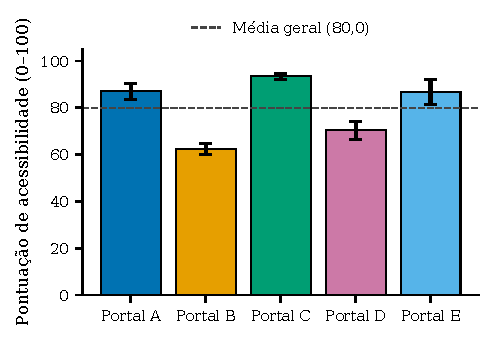
\includegraphics[width=0.48\linewidth]{figures/grafico_barras.pdf}}{\fbox{grafico\_barras.pdf}}
    \hfill
    \IfFileExists{figures/grafico_boxplot.pdf}{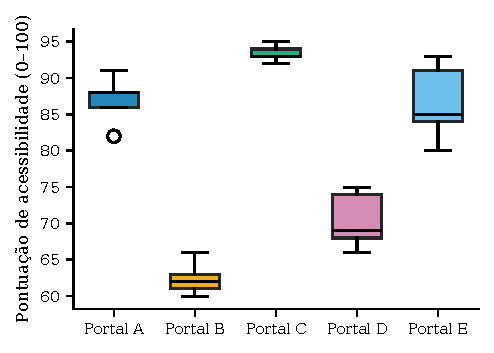
\includegraphics[width=0.48\linewidth]{figures/grafico_boxplot.pdf}}{\fbox{grafico\_boxplot.pdf}}
    \end{tcolorbox}
    \caption{Saídas do kit com os dados de exemplo: barras com média $\pm$ desvio padrão (esquerda) e \textit{boxplot} (direita).}
    \label{fig:exemplos}
\end{figure}

\subsection*{\circulo{5}\hspace{0.4em}Tabela \LaTeX{} gerada automaticamente}
O kit escreve o arquivo \texttt{tabela\_resultados.tex} já no padrão \texttt{booktabs} do Roteiro 01, com vírgula decimal. Nada de digitar números à mão (e errar)!

\begin{codigo}[tex]{tabela\_resultados.tex}
\begin{table}[htbp]
  \caption{Estatísticas descritivas de acessibilidade por portal}
  \label{tab:resultados}
  \centering
  \begin{tabular}{lrrrrr}
    \toprule
    \textbf{Portal} & \textbf{n} & \textbf{Média} & \textbf{DP} & \textbf{Mín.} & \textbf{Máx.} \\
    \midrule
    Portal A & 5 & 87,00 & 3,32 & 82,00 & 91,00 \\
    ...
    \bottomrule
  \end{tabular}
\end{table}
\end{codigo}

% =====================================================
% 7. ESCOLHENDO O GRÁFICO CERTO
% =====================================================
\section{Escolhendo o gráfico certo para a sua pergunta}\label{sec:grafico}

O tipo de gráfico é decidido pela \textbf{pergunta de pesquisa}, não pela estética. Use a tabela abaixo como guia. Se precisar de um gráfico diferente das barras e do \textit{boxplot}, adapte os Blocos 3 e 4 trocando a função do \texttt{matplotlib} (peça ajuda aos professores!).

\begin{center}
\small
\renewcommand{\arraystretch}{1.5}
\rowcolors{2}{fundo}{white}
\begin{tabularx}{\linewidth}{YP{3.9cm}P{3.6cm}}
\cabecalho \cab{A pergunta da pesquisa é\ldots} & \cab{Gráfico indicado} & \cab{Função \texttt{matplotlib}} \\
Qual grupo tem o maior/menor valor médio? & {\color{azulMedio}\faChartBar}\ Barras com erro & \texttt{ax.bar(..., yerr=...)} \\
Os valores de cada grupo são estáveis ou muito espalhados? & {\color{azulMedio}\faGripLinesVertical}\ \textit{Boxplot} & \texttt{ax.boxplot(...)} \\
Como a métrica evoluiu ao longo do tempo/das semanas? & {\color{azulMedio}\faChartLine}\ Linha & \texttt{ax.plot(x, y, marker="o")} \\
Existe relação entre duas métricas (ex.: tempo $\times$ nota)? & {\color{azulMedio}\faBraille}\ Dispersão & \texttt{ax.scatter(x, y)} \\
Como as respostas se distribuem numa escala Likert (1 a 5)? & {\color{azulMedio}\faAlignLeft}\ Barras horizontais empilhadas & \texttt{ax.barh(..., left=...)} \\
\end{tabularx}
\end{center}

\begin{atencao}{Evite em artigos científicos}
Gráficos de \textbf{pizza} (difíceis de comparar com mais de 3 fatias), efeitos \textbf{3D}, sombras, fundos coloridos e \textbf{eixo Y de barras que não começa em zero} (exagera visualmente as diferenças).
\end{atencao}

% =====================================================
% 8. LEVANDO PARA O OVERLEAF
% =====================================================
\section{Levando os resultados para o Overleaf}\label{sec:overleaf}

\begin{enumerate}[label={\protect\circulo[roxo]{\arabic*}}]
    \item No projeto do Overleaf (Roteiro 01), clique no ícone \botao{\faUpload\ Upload} e envie \texttt{grafico\_barras.pdf} (e/ou \texttt{grafico\_boxplot.pdf}) e \texttt{tabela\_resultados.tex};
    \item Na seção de \textbf{Resultados} do \texttt{main.tex}, insira a figura e a tabela:
\end{enumerate}

\begin{codigo}[tex]{main.tex (trecho)}
\section{Resultados e Discussão}

A Figura~\ref{fig:acessibilidade} apresenta a pontuação média de
acessibilidade de cada portal, e a Tabela~\ref{tab:resultados}
detalha as estatísticas descritivas das cinco rodadas de auditoria.

\begin{figure}[htbp]
  \centering
  \includegraphics[width=\columnwidth]{grafico_barras.pdf}
  \caption{Pontuação média de acessibilidade por portal
           (barras de erro: desvio padrão; n = 5 rodadas).}
  \label{fig:acessibilidade}
\end{figure}

\input{tabela_resultados}
\end{codigo}

\begin{sucesso}{Descrever os resultados: interpretar, e não repetir}
O texto não deve narrar a tabela linha por linha. Destaque o \textbf{padrão}, o \textbf{contraste} e o \textbf{significado} para a comunidade atendida pela ação extensionista.\par\vspace{4pt}
\begin{tcbraster}[raster columns=2, raster equal height, raster column skip=8pt]
\begin{tcolorbox}[enhanced, colback=white, colframe=vermelho!35, boxrule=0.6pt, arc=6pt, fontupper=\small\raggedright]
{\color{vermelho}\faTimesCircle\ \textbf{Fraco}}\par
\textit{``O Portal A teve 87, o Portal B teve 62,4, o Portal C teve 93,4, o Portal D teve 70,4 e o Portal E teve 86,6.''}
\end{tcolorbox}
\begin{tcolorbox}[enhanced, colback=white, colframe=verdeVivo!45, boxrule=0.6pt, arc=6pt, fontupper=\small\raggedright]
{\color{verdeVivo}\faCheckCircle\ \textbf{Adequado}}\par
\textit{``Como mostra a Figura 1, três dos cinco portais superaram a média geral (80,0 pontos), com destaque para o Portal C (93,4 $\pm$ 1,1). Os Portais B e D ficaram abaixo de 71 pontos, o que indica barreiras de acesso relevantes para pessoas que usam leitores de tela.''}
\end{tcolorbox}
\end{tcbraster}
\end{sucesso}

\begin{dica}{PDF ou PNG?}
Prefira sempre o \textbf{PDF} (vetorial): textos e linhas continuam nítidos em qualquer zoom e o arquivo é leve. Use o \textbf{PNG em 300 dpi} apenas quando o gráfico tiver milhares de pontos (o PDF ficaria pesado) ou para slides e pôsteres. \textbf{Nunca} use captura de tela (\textit{print}) de um gráfico no artigo.
\end{dica}

% =====================================================
% 9. BOAS PRÁTICAS E ERROS COMUNS
% =====================================================
\section{Boas práticas e erros comuns}\label{sec:erros}

\subsection{Checklist de uma figura científica de qualidade}
\begin{itemize}
    \item \textbf{Sem título dentro da imagem:} no artigo, quem faz esse papel é o \texttt{\textbackslash caption\{\}} --- o kit já remove o título;
    \item \textbf{Eixos com nome e unidade:} ``Tempo de carregamento (s)'', e não apenas ``tempo'';
    \item \textbf{Letras legíveis:} figura gerada na largura de uma coluna (3,33 pol.) e incluída com \texttt{width=\textbackslash columnwidth};
    \item \textbf{Cores acessíveis:} o kit usa a paleta Okabe--Ito, distinguível por pessoas com daltonismo --- coerente com uma disciplina extensionista!
    \item \textbf{Legenda informativa:} a \texttt{\textbackslash caption} deve dizer o que as barras de erro representam e quantas observações existem ($n$);
    \item \textbf{Reprodutibilidade:} guarde o \texttt{.csv} e o notebook junto com o projeto (por exemplo, em uma pasta \texttt{dados/} no Overleaf).
\end{itemize}

\subsection{Erros comuns e como resolver}
\begin{center}
\small
\renewcommand{\arraystretch}{1.5}
\rowcolors{2}{fundo}{white}
\begin{tabularx}{\linewidth}{P{4.3cm}YY}
\cabecalho \cab{Mensagem / sintoma} & \cab{Causa provável} & \cab{Solução} \\
\texttt{NameError: name 'pd' is not defined} & A célula de importação (ou outra anterior) não foi executada & \botao{Ambiente de execução}\seta\botao{Executar tudo} \\
\texttt{[aviso] ... não encontrado} & O \texttt{.csv} não foi enviado, tem outro nome ou a sessão foi reiniciada & Envie o arquivo pelo painel \faFolder\ e confira \texttt{ARQUIVO\_DADOS} \\
\texttt{KeyError: 'acessibilidade'} & O nome da coluna na configuração não existe no CSV & Copie o nome exato exibido por \texttt{df.head()} (maiúsculas e espaços contam) \\
\texttt{SyntaxError} & Aspas não fechadas ou símbolo apagado na configuração & Compare com o exemplo ``Certo'' da Seção~\ref{sec:python} \\
O CSV é lido como \textbf{uma única coluna} & O separador é \texttt{;} (Excel em português) & Use \texttt{SEPARADOR = ";"} e \texttt{DECIMAL = ","} \\
\texttt{TypeError} / \texttt{agg function failed} & Há texto na coluna da métrica (ex.: \texttt{"2,2 s"}, \texttt{"N/A"}) & Deixe apenas números na coluna; células vazias são aceitas \\
Acentos aparecem como \texttt{é} & Codificação do arquivo diferente de UTF-8 & Acrescente \texttt{encoding="latin-1"} ao \texttt{pd.read\_csv(...)} \\
Letras minúsculas no PDF do artigo & Figura gerada grande e reduzida pelo \LaTeX{} & Mantenha \texttt{figsize=(3.33, 2.3)} e \texttt{width=\textbackslash columnwidth} \\
\end{tabularx}
\end{center}

% =====================================================
% 10. ATIVIDADE PRÁTICA
% =====================================================
\section{Atividade prática em laboratório}\label{sec:atividade}

Cada dupla (ou estudante individual) deverá executar o roteiro abaixo:

\begin{painel}{\faTasks}{Passo a passo da atividade de hoje}
\begin{enumerate}[label={\protect\circulo{\arabic*}}, leftmargin=2.4em]
    \item \textbf{Aquecimento:} criar o notebook \texttt{aquecimento.ipynb} e executar as 4 células da Seção~\ref{sec:aquecimento}, incluindo o erro proposital.
    \item \textbf{Execução com os dados de exemplo:} abrir o kit no Colab, salvar uma cópia no Drive, executar todas as células e baixar os 5 arquivos gerados.
    \item \textbf{Preparação dos dados da dupla:} organizar os dados do seu tema (ou um conjunto piloto, se a coleta ainda estiver em andamento) no formato ``uma linha por medição'', com pelo menos \textbf{2 grupos} e \textbf{3 observações por grupo}, e exportar como \texttt{.csv}.
    \item \textbf{Adaptação do kit:} enviar o \texttt{.csv} ao Colab e ajustar a célula \textbf{CONFIGURAÇÃO} (arquivo, colunas e rótulo do eixo com unidade).
    \item \textbf{Escolha do gráfico:} justificar, com base na Seção~\ref{sec:grafico}, qual gráfico responde melhor à pergunta de pesquisa da dupla.
    \item \textbf{Integração no Overleaf:} enviar o gráfico em PDF e o \texttt{tabela\_resultados.tex} e inseri-los na seção de Resultados.
    \item \textbf{Redação interpretativa:} escrever um parágrafo de Resultados que cite a figura e a tabela (\texttt{Figura\textasciitilde\textbackslash ref\{...\}}, \texttt{Tabela\textasciitilde\textbackslash ref\{...\}}) e \textbf{interprete} o padrão observado.
    \item \textbf{Registro no Painel de Equipes:} atualizar o link de leitura (\texttt{/read/}) do Overleaf no Dashboard da disciplina e anexar o link do notebook (\botao{Compartilhar}\seta\textit{Qualquer pessoa com o link: Leitor}).
\end{enumerate}
\end{painel}

\vspace{0.6em}

\begin{tcolorbox}[enhanced, breakable, colback=verdeVivo!5, colframe=verdeVivo!30, boxrule=0.6pt, arc=8pt, left=14pt, right=14pt, top=10pt, bottom=10pt]
{\color{verde}\bfseries\large\faClipboardCheck\hspace{0.5em}Checklist de verificação da entrega}\par\vspace{4pt}
\begin{itemize}[label={\caixaMarcar}, itemsep=0.4em]
    \item Notebook do kit executado no Colab com os dados de exemplo, sem erros;
    \item \texttt{.csv} da dupla no formato ``uma linha por medição'' ($\geq$ 2 grupos, $\geq$ 3 observações por grupo);
    \item Gráfico exportado em \textbf{PDF}, sem título interno e com eixo identificado com unidade;
    \item Tipo de gráfico coerente com a pergunta de pesquisa (Seção~\ref{sec:grafico});
    \item Figura e \texttt{tabela\_resultados.tex} inseridas no Overleaf, compilando sem erros;
    \item Parágrafo de Resultados com citação cruzada e interpretação (não apenas repetição dos números);
    \item Links do Overleaf (\texttt{/read/}) e do Colab registrados no Painel de Equipes.
\end{itemize}
\end{tcolorbox}

\vfill
\begin{center}
    \footnotesize\color{suave}
    Instituto Federal de Santa Catarina (IFSC) — Câmpus Garopaba\\
    Rodovia SC-434, km 04 — Bairro Campo D'Una, Garopaba - SC, CEP 88495-000\\
    \url{https://www.ifsc.edu.br/garopaba}
\end{center}

\end{document}
